\documentclass[11pt, oneside, dvipdfmx]{book}
\newcommand{\folder}{/usr/local/share/texmf}
%Page setting
\setlength{\textwidth}{460pt}
\setlength{\topmargin}{-1truemm}
\setlength{\textheight}{650pt}
\setlength{\oddsidemargin}{-0.2truemm}
\setlength{\evensidemargin}{-0.2truemm}

%%%%%%%%%%%%
% 	 UsePackege	%
%%%%%%%%%%%%
\usepackage{amssymb}
\usepackage{amsmath}
\usepackage{amsthm}
\usepackage{ascmac}
\usepackage{lscape}
\usepackage{pifont}
\usepackage{cite}
\usepackage{ifthen}
\usepackage{framed}
\usepackage{mathrsfs}
\usepackage{booktabs}
\usepackage{algorithm}
\usepackage{algorithmic}
\usepackage{comment}
\usepackage{longtable}
% Font
%%%%%%%%%%%%%%
% 	Bold Number	%
%%%%%%%%%%%%%%
\newcommand{\bzero}{{\bf 0}}
\newcommand{\bone}{{\bf 1}}
%%%%%%%%%%%%%%
% 	Bold English	%
%%%%%%%%%%%%%%
% a
\newcommand{\ba}{{\mbox{\boldmath$a$}}}
\newcommand{\bA}{{\mbox{\boldmath$A$}}}
\newcommand{\sba}{{\mbox{\scriptsize\boldmath $a$}}}
% b
\newcommand{\bb}{{\mbox{\boldmath$b$}}}
\newcommand{\bB}{{\mbox{\boldmath$B$}}}
\newcommand{\sbb}{{\mbox{\scriptsize\boldmath $b$}}}
% c
\newcommand{\bc}{{\mbox{\boldmath$c$}}}
\newcommand{\bC}{{\mbox{\boldmath$C$}}}
\newcommand{\sbC}{{\mbox{\scriptsize\boldmath $C$}}}
\newcommand{\sbc}{{\mbox{\scriptsize\boldmath $c$}}}
% d
\newcommand{\bd}{{\mbox{\boldmath$d$}}}
\newcommand{\bD}{{\mbox{\boldmath$D$}}}
\newcommand{\sbd}{{\mbox{\scriptsize\boldmath $d$}}}
% e
\newcommand{\be}{{\mbox{\boldmath$e$}}}
\newcommand{\bE}{{\mbox{\boldmath$E$}}}
\newcommand{\sbe}{{\mbox{\scriptsize\boldmath $e$}}}
% f
\newcommand{\bbf}{{\mbox{\boldmath$f$}}}
\newcommand{\bF}{{\mbox{\boldmath$F$}}}
% g
\newcommand{\bg}{{\mbox{\boldmath$g$}}}
\newcommand{\bG}{{\mbox{\boldmath$G$}}}
% h
\newcommand{\bh}{{\mbox{\boldmath$h$}}}
\newcommand{\bH}{{\mbox{\boldmath$H$}}}
\newcommand{\sbH}{{\mbox{\scriptsize\boldmath$H$}}}
\newcommand{\sbh}{{\mbox{\scriptsize\boldmath$h$}}}
% i
\newcommand{\bi}{{\mbox{\boldmath$i$}}}
\newcommand{\sbi}{{\mbox{\scriptsize \boldmath$i$}}}
\newcommand{\bI}{{\mbox{\boldmath$I$}}}
% i
\newcommand{\bj}{{\mbox{\boldmath$j$}}}
\newcommand{\sbj}{{\mbox{\scriptsize \boldmath$j$}}}
\newcommand{\bJ}{{\mbox{\boldmath$J$}}}
% k
\newcommand{\bk}{{\mbox{\boldmath$k$}}}
\newcommand{\bK}{{\mbox{\boldmath$K$}}}
% l
%\newcommand{\ell}{{\mbox{\boldmath $l$}}}
\newcommand{\bl}{{\mbox{\boldmath$l$}}}
\newcommand{\bL}{{\mbox{\boldmath$L$}}}
% m
\newcommand{\bm}{{\mbox{\boldmath$m$}}}
\newcommand{\sbm}{{\mbox{\scriptsize \boldmath$m$}}}
\newcommand{\bM}{{\mbox{\boldmath$M$}}}
% n
\newcommand{\bn}{{\mbox{\boldmath$n$}}}
\newcommand{\bN}{{\mbox{\boldmath$N$}}}
\newcommand{\sbn}{{\mbox{\scriptsize \boldmath$n$}}}
\newcommand{\sbN}{{\mbox{\scriptsize\boldmath $N$}}}
% o
\newcommand{\bo}{{\mbox{\boldmath$o$}}}
\newcommand{\bO}{{\mbox{\boldmath$O$}}}
% p
\newcommand{\bp}{{\mbox{\boldmath$p$}}}
\newcommand{\bP}{{\mbox{\boldmath$P$}}}
\newcommand{\sbp}{{\mbox{\scriptsize \boldmath$p$}}}
% q
\newcommand{\bq}{{\mbox{\boldmath$q$}}}
\newcommand{\bQ}{{\mbox{\boldmath$Q$}}}
% r
\newcommand{\br}{{\mbox{\boldmath$r$}}}
\newcommand{\bR}{{\mbox{\boldmath$R$}}}
\newcommand{\sbr}{{\mbox{\scriptsize\boldmath$r$}}}
% s
\newcommand{\bs}{{\mbox{\boldmath$s$}}}
\newcommand{\sbs}{{\mbox{\scriptsize \boldmath$s$}}}
\newcommand{\bS}{{\mbox{\boldmath$S$}}}
% t
\newcommand{\bt}{{\mbox{\boldmath$t$}}}
\newcommand{\bT}{{\mbox{\boldmath$T$}}}
% u
\newcommand{\bu}{{\mbox{\boldmath$u$}}}
\newcommand{\bU}{{\mbox{\boldmath$U$}}}
\newcommand{\sbu}{{\mbox{\scriptsize\boldmath $u$}}}
% v
\newcommand{\bv}{{\mbox{\boldmath$v$}}}
\newcommand{\bV}{{\mbox{\boldmath$V$}}}
% w
\newcommand{\bw}{{\mbox{\boldmath$w$}}}
\newcommand{\bW}{{\mbox{\boldmath$W$}}}
\newcommand{\sbW}{{\mbox{\scriptsize\boldmath $W$}}}
\newcommand{\sbw}{{\mbox{\scriptsize\boldmath $w$}}}
% x
\newcommand{\bx}{{\mbox{\boldmath$x$}}}
\newcommand{\bX}{{\mbox{\boldmath$X$}}}
\newcommand{\sbx}{{\mbox{\scriptsize\boldmath $x$}}}
\newcommand{\sbX}{{\mbox{\scriptsize\boldmath $X$}}}
%y
\newcommand{\by}{{\mbox{\boldmath$y$}}}
\newcommand{\bY}{{\mbox{\boldmath$Y$}}}
\newcommand{\sby}{{\mbox{\scriptsize\boldmath $y$}}}
\newcommand{\sbY}{{\mbox{\scriptsize\boldmath $Y$}}}
%z
\newcommand{\bz}{{\mbox{\boldmath$z$}}}
\newcommand{\bZ}{{\mbox{\boldmath$Z$}}}
\newcommand{\sbz}{{\mbox{\scriptsize\boldmath$z$}}}
\newcommand{\sbZ}{{\mbox{\scriptsize\boldmath$Z$}}}


%%%%%%%%%%%
% 	Bold Grik	%
%%%%%%%%%%%
% alpha
\newcommand{\balpha}{{\mbox{\boldmath$\alpha$}}}
\newcommand{\sbalpha}{{\mbox{\scriptsize\boldmath$\alpha$}}}
% beta
\newcommand{\bbeta}{{\mbox{\boldmath$\beta$}}}
\newcommand{\sbbeta}{{\mbox{\scriptsize\boldmath$\beta$}}}
% gamma
\newcommand{\bgamma}{{\mbox{\boldmath$\gamma$}}}
\newcommand{\bGamma}{{\mbox{\boldmath$\Gamma$}}}
\newcommand{\sbgamma}{{\mbox{\scriptsize\boldmath$\gamma$}}}
% delta
\newcommand{\bdelta}{{\mbox{\boldmath$\delta$}}}
\newcommand{\bDelta}{{\mbox{\boldmath$\Delta$}}}
\newcommand{\sbdelta}{{\mbox{\scriptsize\boldmath$\delta$}}}
% epsilon
\newcommand{\bepsilon}{{\mbox{\boldmath$\epsilon$}}}
\newcommand{\bvarepsilon}{{\mbox{\boldmath$\varepsilon$}}}
\newcommand{\sbvarepsilon}{{\mbox{\scriptsize\boldmath$\varepsilon$}}}
% zeta
\newcommand{\bzeta}{{\mbox{\boldmath$\zeta$}}}
% eta
\newcommand{\etab}{{\mbox{\boldmath$\eta$}}}
% theta
\newcommand{\btheta}{{\mbox{\boldmath$\theta$}}}
\newcommand{\bTheta}{{\mbox{\boldmath$\Theta$}}}
\newcommand{\bvartheta}{{\mbox{\boldmath$\vartheta$}}}
% iota
\newcommand{\biota}{{\mbox{\boldmath$\iota$}}}
\newcommand{\sbiota}{{\mbox{\scriptsize\boldmath$\iota$}}}
% kappa
\newcommand{\bkappa}{{\mbox{\boldmath$\kappa$}}}
% lambda
\newcommand{\blambda}{{\mbox{\boldmath$\lambda$}}}
\newcommand{\bLambda}{{\mbox{\boldmath$\Lambda$}}}
% mu
\newcommand{\bmu}{{\mbox{\boldmath$\mu$}}}
\newcommand{\sbmu}{{\mbox{\scriptsize\boldmath$\mu$}}}
% nu
\newcommand{\bnu}{{\mbox{\boldmath$\nu$}}}
\newcommand{\sbnu}{{\mbox{\scriptsize\boldmath$\nu$}}}
% xi
\newcommand{\bxi}{{\mbox{\boldmath$\xi$}}}
\newcommand{\bXi}{{\mbox{\boldmath$\Xi$}}}
% pi
\newcommand{\bpi}{{\mbox{\boldmath$\pi$}}}
\newcommand{\bPi}{{\mbox{\boldmath$\Pi$}}}
\newcommand{\bvarpi}{{\mbox{\boldmath$\varpi$}}}
% rho
\newcommand{\brho}{{\mbox{\boldmath$\rho$}}}
\newcommand{\bvarrho}{{\mbox{\boldmath$\varrho$}}}
% sigma
\newcommand{\bsigma}{{\mbox{\boldmath$\sigma$}}}
\newcommand{\bSigma}{{\mbox{\boldmath$\Sigma$}}}
\newcommand{\bvarsigma}{{\mbox{\boldmath$\varsigma$}}}
% tau
\newcommand{\btau}{{\mbox{\boldmath$\tau$}}}
% upsilon
\newcommand{\bupsilon}{{\mbox{\boldmath$\upsilon$}}}
\newcommand{\bUpsilon}{{\mbox{\boldmath$\Upsilon$}}}
% phi
\newcommand{\bphi}{{\mbox{\boldmath$\phi$}}}
\newcommand{\bPhi}{\mathbf \Phi}
\newcommand{\bvarphi}{{\mbox{\boldmath$\varphi$}}}
% chi
\newcommand{\bchi}{{\mbox{\boldmath$\chi$}}}
% psi
\newcommand{\bpsi}{{\mbox{\boldmath$\psi$}}}
\newcommand{\bPsi}{\mathbf \Psi}
% omega
\newcommand{\bomega}{{\mbox{\boldmath$\omega$}}}
\newcommand{\bOmega}{{\mbox{\boldmath$\Omega$}}}
% nabla
\newcommand{\bnabla}{{\mbox{\boldmath$\nabla$}}}

% calligraphic letters
\newcommand{\cA}{{\cal A}}
\newcommand{\cB}{{\cal B}}
\newcommand{\cC}{{\cal C}}
\newcommand{\cD}{{\cal D}}
\newcommand{\cE}{{\cal E}}
\newcommand{\cF}{{\cal F}}
\newcommand{\cG}{{\cal G}}
\newcommand{\cH}{{\cal H}}
\newcommand{\cI}{{\cal I}}
\newcommand{\cJ}{{\cal J}}
\newcommand{\cK}{{\cal K}}
\newcommand{\cL}{{\cal L}}
\newcommand{\cM}{{\cal M}}
\newcommand{\cN}{{\cal N}}
\newcommand{\cO}{{\cal O}}
\newcommand{\cP}{{\cal P}}
\newcommand{\cQ}{{\cal Q}}
\newcommand{\cR}{{\cal R}}
\newcommand{\cS}{{\cal S}}
\newcommand{\cT}{{\cal T}}
\newcommand{\cU}{{\cal U}}
\newcommand{\cV}{{\cal V}}
\newcommand{\cW}{{\cal W}}
\newcommand{\cX}{{\cal X}}
\newcommand{\cY}{{\cal Y}}
\newcommand{\cZ}{{\cal Z}}
% calligraphic letters
\newcommand{\mA}{{\mathscr A}}
\newcommand{\mB}{{\mathscr B}}
\newcommand{\mC}{{\mathscr C}}
\newcommand{\mD}{{\mathscr D}}
\newcommand{\mE}{{\mathscr E}}
\newcommand{\mF}{{\mathscr F}}
\newcommand{\mG}{{\mathscr G}}
\newcommand{\mH}{{\mathscr H}}
\newcommand{\mI}{{\mathscr I}}
\newcommand{\mJ}{{\mathscr J}}
\newcommand{\mK}{{\mathscr K}}
\newcommand{\mL}{{\mathscr L}}
\newcommand{\mM}{{\mathscr M}}
\newcommand{\mN}{{\mathscr N}}
\newcommand{\mO}{{\mathscr O}}
\newcommand{\mP}{{\mathscr P}}
\newcommand{\mQ}{{\mathscr Q}}
\newcommand{\mR}{{\mathscr R}}
\newcommand{\mS}{{\mathscr S}}
\newcommand{\mT}{{\mathscr T}}
\newcommand{\mU}{{\mathscr U}}
\newcommand{\mV}{{\mathscr V}}
\newcommand{\mW}{{\mathscr W}}
\newcommand{\mX}{{\mathscr X}}
\newcommand{\mY}{{\mathscr Y}}
\newcommand{\mZ}{{\mathscr Z}}
% calligraphic letters
\newcommand{\bbA}{{\mathbb A}}
\newcommand{\bbB}{{\mathbb B}}
\newcommand{\bbC}{\mathbb{C}}
\newcommand{\bbD}{\mathbb{D}}
\newcommand{\bbE}{{\mathbb E}}
\newcommand{\bbF}{{\mathbb F}}
\newcommand{\bbG}{{\mathbb G}}
\newcommand{\bbH}{{\mathbb H}}
\newcommand{\bbI}{{\mathbb I}}
\newcommand{\bbJ}{{\mathbb J}}
\newcommand{\bbK}{{\mathbb K}}
\newcommand{\bbL}{\mathbb{L}}
\newcommand{\bbM}{{\mathbb M}}
\newcommand{\bbN}{\mathbb{N}}
\newcommand{\bbO}{{\mathbb O}}
\newcommand{\bbP}{\mathbb{P}}
\newcommand{\bbQ}{{\mathbb Q}}
\newcommand{\bbR}{\mathbb{R}}
\newcommand{\bbS}{\mathbb{S}}
\newcommand{\bbT}{{\mathbb T}}
\newcommand{\bbU}{{\mathbb U}}
\newcommand{\bbV}{\mathbb{V}}
\newcommand{\bbW}{{\mathbb W}}
\newcommand{\bbX}{\mathbb{X}}
\newcommand{\bbY}{\mathbb{Y}}
\newcommand{\bbZ}{{\mathbb Z}}
%%%%%%%%%%%%%%
% 	Tilde English	%
%%%%%%%%%%%%%%
% a
\newcommand{\tila}{\tilde{a}}
\newcommand{\tilA}{\tilde{A}}
% b
\newcommand{\tilb}{\tilde{b}}
\newcommand{\tilB}{\tilde{B}}
% c
\newcommand{\tilc}{\tilde{c}}
\newcommand{\tilC}{\tilde{C}}
% d
\newcommand{\tild}{\tilde{d}}
\newcommand{\tilD}{\tilde{D}}
% e
\newcommand{\tile}{\tilde{e}}
\newcommand{\tilE}{\tilde{E}}
% f
\newcommand{\tilf}{\tilde{f}}
\newcommand{\tilF}{\tilde{F}}
% g
\newcommand{\tilg}{\tilde{g}}
\newcommand{\tilG}{\tilde{G}}
% h
\newcommand{\tilh}{\tilde{h}}
\newcommand{\tilbh}{\tilde\bh}
\newcommand{\tilH}{\tilde{H}}
% i
\newcommand{\tili}{\tilde{i}}
\newcommand{\tilI}{\tilde{I}}
% i
\newcommand{\tilj}{\tilde{j}}
\newcommand{\tilJ}{\tilde{J}}
% k
\newcommand{\tilk}{\tilde{k}}
\newcommand{\tilK}{\tilde{K}}
% l
\newcommand{\till}{\tilde{l}}
\newcommand{\tilL}{\tilde{L}}
% m
\newcommand{\tilm}{\tilde{m}}
\newcommand{\tilM}{\tilde{M}}
% n
\newcommand{\tiln}{\tilde{n}}
\newcommand{\tilN}{\tilde{N}}
% o
\newcommand{\tilo}{\tilde{o}}
\newcommand{\tilO}{\tilde{O}}
% p
\newcommand{\tilp}{\tilde{p}}
\newcommand{\tilP}{\tilde{P}}
% q
\newcommand{\tilq}{\tilde{q}}
\newcommand{\tilQ}{\tilde{Q}}
\newcommand{\tilbq}{\tilde{\bq}}
% r
\newcommand{\tilr}{\tilde{r}}
\newcommand{\tilR}{\tilde{R}}
\newcommand{\tilcR}{\tilde{\cR}}
\newcommand{\tilbr}{\tilde{\br}}
% s
\newcommand{\tils}{\tilde{s}}
\newcommand{\tilS}{\tilde{S}}
% t
\newcommand{\tilt}{\tilde{t}}
\newcommand{\tilT}{\tilde{T}}
% u
\newcommand{\tilu}{\tilde{u}}
\newcommand{\tilU}{\tilde{U}}
% v
\newcommand{\tilv}{\tilde{v}}
\newcommand{\tilV}{\tilde{V}}
% w
\newcommand{\tilw}{\tilde{w}}
\newcommand{\tilW}{\tilde{W}}
% x
\newcommand{\tilx}{\tilde{x}}
\newcommand{\tilbx}{\tilde{\bx}}
\newcommand{\tilX}{\tilde{X}}
\newcommand{\tilbX}{\tilde{\bX}}
%y
\newcommand{\tily}{\tilde{y}}
\newcommand{\tilY}{\tilde{Y}}
\newcommand{\tilby}{\tilde{\by}}
\newcommand{\tilbY}{\tilde{\bY}}
%z
\newcommand{\tilz}{\tilde{z}}
\newcommand{\tilZ}{\tilde{Z}}
\newcommand{\tilbZ}{\tilde{\bZ}}


%%%%%%%%%%%%
%% 	Bold Grik	%
%%%%%%%%%%%%
%% alpha
\newcommand{\tilalpha}{\tilde{\alpha}}
%\newcommand{\sbalpha}{{\mbox{\scriptsize\boldmath$\alpha$}}}
%% beta
\newcommand{\tilbeta}{{\tilde{\beta}}}
%\newcommand{\sbbeta}{{\mbox{\scriptsize\boldmath$\beta$}}}
%% gamma
\newcommand{\tilgamma}{{\tilde{\gamma}}}
%\newcommand{\bGamma}{{\mbox{\boldmath$\Gamma$}}}
%\newcommand{\sbgamma}{{\mbox{\scriptsize\boldmath$\gamma$}}}
%% delta
%\newcommand{\bdelta}{{\mbox{\boldmath$\delta$}}}
%\newcommand{\bDelta}{{\mbox{\boldmath$\Delta$}}}
%\newcommand{\sbdelta}{{\mbox{\scriptsize\boldmath$\delta$}}}
%% epsilon
%\newcommand{\bepsilon}{{\mbox{\boldmath$\epsilon$}}}
%\newcommand{\bvarepsilon}{{\mbox{\boldmath$\varepsilon$}}}
%\newcommand{\sbvarepsilon}{{\mbox{\scriptsize\boldmath$\varepsilon$}}}
%% zeta
%\newcommand{\bzeta}{{\mbox{\boldmath$\zeta$}}}
%% eta
%\newcommand{\etab}{{\mbox{\boldmath$\eta$}}}
%% theta
%\newcommand{\btheta}{{\mbox{\boldmath$\theta$}}}
%\newcommand{\bTheta}{{\mbox{\boldmath$\Theta$}}}
%\newcommand{\bvartheta}{{\mbox{\boldmath$\vartheta$}}}
%% iota
%\newcommand{\biota}{{\mbox{\boldmath$\iota$}}}
%\newcommand{\sbiota}{{\mbox{\scriptsize\boldmath$\iota$}}}
%% kappa
%\newcommand{\bkappa}{{\mbox{\boldmath$\kappa$}}}
%% lambda
%\newcommand{\blambda}{{\mbox{\boldmath$\lambda$}}}
%\newcommand{\bLambda}{{\mbox{\boldmath$\Lambda$}}}
%% mu
%\newcommand{\bmu}{{\mbox{\boldmath$\mu$}}}
%\newcommand{\sbmu}{{\mbox{\scriptsize\boldmath$\mu$}}}
%% nu
%\newcommand{\bnu}{{\mbox{\boldmath$\nu$}}}
%\newcommand{\sbnu}{{\mbox{\scriptsize\boldmath$\nu$}}}
%% xi
%\newcommand{\bxi}{{\mbox{\boldmath$\xi$}}}
%\newcommand{\bXi}{{\mbox{\boldmath$\Xi$}}}
%% pi
%\newcommand{\bpi}{{\mbox{\boldmath$\pi$}}}
%\newcommand{\bPi}{{\mbox{\boldmath$\Pi$}}}
%\newcommand{\bvarpi}{{\mbox{\boldmath$\varpi$}}}
%% rho
%\newcommand{\brho}{{\mbox{\boldmath$\rho$}}}
%\newcommand{\bvarrho}{{\mbox{\boldmath$\varrho$}}}
%% sigma
%\newcommand{\bsigma}{{\mbox{\boldmath$\sigma$}}}
%\newcommand{\bSigma}{{\mbox{\boldmath$\Sigma$}}}
%\newcommand{\bvarsigma}{{\mbox{\boldmath$\varsigma$}}}
% tau
\newcommand{\tiltau}{{\mbox{$\tilde{\tau}$}}}
%% upsilon
%\newcommand{\bupsilon}{{\mbox{\boldmath$\upsilon$}}}
%\newcommand{\bUpsilon}{{\mbox{\boldmath$\Upsilon$}}}
%% phi
%\newcommand{\bphi}{{\mbox{\boldmath$\phi$}}}
%\newcommand{\bPhi}{\mathbf \Phi}
%\newcommand{\bvarphi}{{\mbox{\boldmath$\varphi$}}}
%% chi
%\newcommand{\bchi}{{\mbox{\boldmath$\chi$}}}
%% psi
%\newcommand{\bpsi}{{\mbox{\boldmath$\psi$}}}
%\newcommand{\bPsi}{\mathbf \Psi}
%% omega
%\newcommand{\bomega}{{\mbox{\boldmath$\omega$}}}
%\newcommand{\bOmega}{{\mbox{\boldmath$\Omega$}}}

%%%%%%%%%%%%%%
% 	Tilde English	%
%%%%%%%%%%%%%%
% a
\newcommand{\bara}{\bar{a}}
\newcommand{\barA}{\bar{A}}
% b
\newcommand{\barb}{\bar{b}}
\newcommand{\barB}{\bar{B}}
% c
\newcommand{\barc}{\bar{c}}
\newcommand{\barC}{\bar{C}}
% d
\newcommand{\bard}{\bar{d}}
\newcommand{\barD}{\bar{D}}
% e
\newcommand{\bare}{\bar{e}}
\newcommand{\barE}{\bar{E}}
% f
\newcommand{\barbf}{\bar{f}}
\newcommand{\barF}{\bar{F}}
% g
\newcommand{\barg}{\bar{g}}
\newcommand{\barG}{\bar{G}}
% h
\newcommand{\barh}{\bar{h}}
\newcommand{\barbh}{\bar\bh}
\newcommand{\barH}{\bar{H}}
% i
\newcommand{\bari}{\bar{i}}
\newcommand{\barI}{\bar{I}}
% i
\newcommand{\barj}{\bar{j}}
\newcommand{\barJ}{\bar{J}}
% k
\newcommand{\bark}{\bar{k}}
\newcommand{\barK}{\bar{K}}
% l
\newcommand{\barl}{\bar{l}}
\newcommand{\barL}{\bar{L}}
% m
\newcommand{\barm}{\bar{m}}
\newcommand{\barM}{\bar{M}}
% n
\newcommand{\barn}{\bar{n}}
\newcommand{\barN}{\bar{N}}
% o
\newcommand{\baro}{\bar{o}}
\newcommand{\barO}{\bar{O}}
% p
\newcommand{\barp}{\bar{p}}
\newcommand{\barP}{\bar{P}}
% q
\newcommand{\barq}{\bar{q}}
\newcommand{\barQ}{\bar{Q}}
% r
\newcommand{\barr}{\bar{r}}
\newcommand{\barR}{\bar{R}}
% s
\newcommand{\bars}{\bar{s}}
\newcommand{\barS}{\bar{S}}
% t
\newcommand{\bart}{\bar{t}}
\newcommand{\barT}{\bar{T}}
% u
\newcommand{\baru}{\bar{u}}
\newcommand{\barU}{\bar{U}}
% v
\newcommand{\barv}{\bar{v}}
\newcommand{\barV}{\bar{V}}
% w
\newcommand{\barw}{\bar{w}}
\newcommand{\barW}{\bar{W}}
\newcommand{\barbw}{\bar{\bw}}
% x
\newcommand{\barx}{\bar{x}}
\newcommand{\barX}{\bar{X}}
%y
\newcommand{\bary}{\bar{y}}
\newcommand{\barY}{\bar{Y}}
%z
\newcommand{\barz}{\bar{z}}
\newcommand{\barZ}{\bar{Z}}
%%%%%%%%%%%%%%
% 	Hat English	%
%%%%%%%%%%%%%%
% a
\newcommand{\hata}{\hat{a}}
\newcommand{\hatA}{\hat{A}}
% b
\newcommand{\hatb}{\hat{b}}
\newcommand{\hatB}{\hat{B}}
% c
\newcommand{\hatc}{\hat{c}}
\newcommand{\hatC}{\hat{C}}
\newcommand{\hatbc}{\hat{\bc}}
% d
\newcommand{\hatd}{\hat{d}}
\newcommand{\hatD}{\hat{D}}
% e
\newcommand{\hate}{\hat{e}}
\newcommand{\hatE}{\hat{E}}
% f
\newcommand{\hatbf}{\hat{f}}
\newcommand{\hatF}{\hat{F}}
% g
\newcommand{\hatg}{\hat{g}}
\newcommand{\hatG}{\hat{G}}
% h
\newcommand{\hath}{\hat{h}}
\newcommand{\hatbh}{\hat\bh}
\newcommand{\hatH}{\hat{H}}
% i
\newcommand{\hati}{\hat{i}}
\newcommand{\hatI}{\hat{I}}
% i
\newcommand{\hatj}{\hat{j}}
\newcommand{\hatJ}{\hat{J}}
% k
\newcommand{\hatk}{\hat{k}}
\newcommand{\hatK}{\hat{K}}
% l
\newcommand{\hatl}{\hat{l}}
\newcommand{\hatL}{\hat{L}}
% m
\newcommand{\hatm}{\hat{m}}
\newcommand{\hatM}{\hat{M}}
% n
\newcommand{\hatn}{\hat{n}}
\newcommand{\hatN}{\hat{N}}
% o
\newcommand{\hato}{\hat{o}}
\newcommand{\hatO}{\hat{O}}
% p
\newcommand{\hatp}{\hat{p}}
\newcommand{\hatP}{\hat{P}}
% q
\newcommand{\hatq}{\hat{q}}
\newcommand{\hatQ}{\hat{Q}}
% r
\newcommand{\hatr}{\hat{r}}
\newcommand{\hatR}{\hat{R}}
\newcommand{\hatbr}{\hat{\br}}
% s
\newcommand{\hats}{\hat{s}}
\newcommand{\hatS}{\hat{S}}
% t
\newcommand{\hatt}{\hat{t}}
\newcommand{\hatT}{\hat{T}}
% u
\newcommand{\hatu}{\hat{u}}
\newcommand{\hatU}{\hat{U}}
% v
\newcommand{\hatv}{\hat{v}}
\newcommand{\hatV}{\hat{V}}
% w
\newcommand{\hatw}{\hat{w}}
\newcommand{\hatW}{\hat{W}}
% x
\newcommand{\hatx}{\hat{x}}
\newcommand{\hatX}{\hat{X}}
\newcommand{\hatbX}{\hat{\bX}}
%y
\newcommand{\haty}{\hat{y}}
\newcommand{\hatY}{\hat{Y}}
%z
\newcommand{\hatz}{\hat{z}}
\newcommand{\hatZ}{\hat{Z}}
%%%%%%%%%%%%%%
% 	Tilde English	%
%%%%%%%%%%%%%%
% A
\newcommand{\mathall}{{\rm all}}
\newcommand{\mathand}{{\rm and}}
% B
\newcommand{\BER}{{\rm BER}}
% C
\newcommand{\Cov}{{\rm Cov}}
\newcommand{\conv}{{\rm conv}}
% D
\newcommand{\diver}{\mathrm{div~}}
% E
\newcommand{\eg}{\textit{e.g.}}
\newcommand{\etc}{\textit{etc.}}
\newcommand{\etal}{\textit{et al.}}
\newcommand{\iid}{\textit{i.i.d.}}
\newcommand{\ie}{\textit{i.e.}}
% F
\newcommand{\mathfor}{{\rm for}}
% G
\newcommand{\GF}{{\rm GF}}
\newcommand{\grad}{\mathrm{grad~}}
% I

\newcommand{\mathif}{{\rm if}}
% O
\newcommand{\opt}{{\rm opt}}
\newcommand{\mathor}{{\rm or}}
\newcommand{\mathotherwise}{{\rm otherwise}}
% R
\newcommand{\rot}{\mathrm{rot~}}
% S
\newcommand{\SER}{{\rm SER}}
\newcommand{\st}{~\mathrm{s.t.}~}
% T
%\newcommand{\th}{\mathrm{th}}
% V
\newcommand{\Var}{{\rm Var}}





% Environment
%%%%%%%%%%%%
% 	 Operations 		%
%%%%%%%%%%%%
\DeclareMathOperator{\diag}{diag}
\DeclareMathOperator*{\argmin}{arg~min}
\DeclareMathOperator*{\argmax}{arg~max}
\DeclareMathOperator*{\minmax}{min~max}
\DeclareMathOperator*{\maxmin}{max~min}
\DeclareMathOperator{\lcm}{lcm}
\DeclareMathOperator{\mtxop}{mtx}
\DeclareMathOperator{\vecop}{vec}
\DeclareMathOperator{\sinc}{sinc}
\DeclareMathOperator{\sgn}{sgn}
\DeclareMathOperator{\rank}{rank}
\DeclareMathOperator{\tr}{tr}
\DeclareMathOperator{\sig}{sig}
% New Environment
\newenvironment{MyDefinition}[1]
    {\begin{itembox}[l]{\bf #1}
    \begin{definition}}%
    {\end{definition}
    \end{itembox}}
    
\newenvironment{MyTheorem}
    {\begin{shadebox}
    \bigskip
    \begin{theorem}}%
    {\end{theorem}
    \smallskip
    \end{shadebox}}
 
\newenvironment{MyProof}
    {\begin{boxnote}
    	%\begin{quote}
    %\begin{proof}
    }
    {%\end{proof}
    %\end{quote}
\end{boxnote}}
 
 \newenvironment{MyExample}
 {\begin{shaded}
 		\begin{quote}
 		\begin{example}}%
 		{\end{example}
   \end{quote}
\end{shaded}}
  
\newenvironment{MyLemma}
    {\begin{doublebox}
    \begin{lemma}}%
    {\end{lemma}
    \end{doublebox}}
    

    
% References
%\newcommand{\IEEE_L_COM}{{IEEE} Commun. Lett.~}

\newcommand{\GCOM}{{IEEE} Global Telecommun. Conf.~}
\newcommand{\ICC}{{IEEE} Int. Conf. Commun.~}
\newcommand{\ISIT}{{IEEE} Int. Symp. Infor. Theory~}
\newcommand{\IWSDA}{{IEEE} Int. Workshop Signal Design and Its Applications in Commun.~}
\newcommand{\MILCOM}{{IEEE} Military Commun. Conf.~}
\newcommand{\PIMRC}{{IEEE} Int. Symp. Personal, Indoor and Mobile Radio Commun.~}
\newcommand{\VTC}{{IEEE} Veh. Tech. Conf.~}
\newcommand{\WCNC}{{IEEE} Wireless Commun. Networking Conf.~}
\bibliographystyle{IEEEtran}
% New Theorems
\theoremstyle{definition}
% Theorem style includes plain, definition, and remark
\newtheorem{theorem}{Theorem}
%\newtheorem{algorithm}{Algorithm}
\newtheorem{definition}{Definition}
\newtheorem{example}{Example}
\newtheorem{conjecture}{Conjecture}
\newtheorem{criterion}{Criterion}
\newtheorem{lemma}{Lemma}
\newtheorem{proposition}{Proposition}
\newtheorem{corollary}{Corollary}
\newtheorem{assumption}{Assumption}
\newtheorem{remark}{Remark}
\newtheorem{problem}{Problem}[section]
\usepackage[dvipdfmx]{color}
\usepackage[dvipdfmx]{graphicx}
\usepackage[sectionbib]{chapterbib}
%\renewcommand{\bibname}{参考情報}
\definecolor{shadecolor}{rgb}{0.9,0.9,0.9}
\makeatletter
\def\th@plain{\upshape}
\makeatother

\renewcommand{\theequation}{\arabic{chapter}-\arabic{equation}}
\renewcommand{\thefigure}{\arabic{chapter}-\arabic{figure}}
\usepackage{graphics}
%\setCJKmainfont{SimSun}
\title{``
Time-Varying Periodic Convolutional Codes With Low-Density Parity-Check Matrix'' by 
Alberto Jimenez Felstrom and
Kamil Sh. Zigangiro}
\author{Kwame Ackah Bohulu}
\date{\today}
\begin{document}

\maketitle

\paragraph{Abstract-}
We present a class of convolutional codes defined by a low-density parity-check (LDPC) matrix and an iterative algorithm of the decoding of
these codes. The performance of this decoding is close to the performance
of turbo decoding. Our simulation shows that for the rate $R = 1/2$
binary codes, the performance is substantionally better than for ordinary
convolutional codes with the same decoding complexity per information
bit. As an example, we constructed convolutional codes with memory
$M = 1025, 2049 ~\text{and} ~4097$ showing that we are about $1$ dB from
the capacity limit at a bit-error rate (BER) of $10^{-5}$ and a decoding
complexity of the same magnitude as a Viterbi decoder for codes having
memory $M = 1$


\section{Introduction}
In the 1960's Gallager first introduced LDPC block codes and also studied an iterative decoding algorithm which showed promise in acheiving low error probabilities at high data rates with very reasonable costs.

Iterative decoding has since gained a lot of attention[2] -[4] especially with the recent simulation results [5],[6] which revealed that LDPC codes have performance close to the Shannon limit, which is also similar to turbo codes.

This paper focuses on the convolutional version of LDPC codes. It is revealed that they perform better than block codes of the same length and have a much regular structure which makes encoder and decoder implementation easier. Decoding can also be sped up by using a pipeline structure involving several processors.

Due to statistical dependence, a mathematical performance analysis of iterative decoding is generally difficult. A successful atempt of LDPC iterative decoding was made by V. Zyablov and M. Pinsker [7]. They were able to proove that the number of corrected errors increases linearly with block length. In practise however BER is of more interest and as far as the authours know, most of the BER analysis that exists is based on simulation results.


\section{LDPC Block Codes and Iterative  Decoding}
An $(N,J,K)$ LDPC matrix $\bH$ of a block code over GF(2) is a matrix with $N$ columns, each column having weight $J$ and each row having weight $K$. In general 
$\bH$ can be represented as shown in \ref{1}



\begin{equation}
\bH
=
\begin{bmatrix}
    \bM \bP_{1} \\
    \bM \bP_{2}  \\
    \vdots  \\
    \bM \bP_{J} 
\end{bmatrix}
\label{1}
\end{equation}


where 
\begin{description}
\item [$\bM$] is an $\frac{N}{K} \times N$ matrix made up of $K$ concatenated $\frac{N}{K}$ unity matrices $\bI$
\item [$\bP$] is any $N \times N$ permutation matrix, so $\bH$ has $\frac{NJ}{K}$
\end{description}

The rate $R$ of the code is $R \geq 1- \frac{J}{K}$ since not all the rows are linearly independent. It is worth mentioning that in principle, it is possible to construct LDPC codes with different column weight $J$ and or row weights $K$

Using a slightly different construction, Gallager[1] proved the existence of LDPC codes whose minimum distance $d_{min}$ increases linearly with block length $N$ when $J>2$. Furthermore, he proved that
for $J > 2$, the ratio of the minimum distance to the code length of a
typical code limits to a nonzero constant $\alpha$, which is dependent on
the selection $J$ and $K$

We continue by considering the case where an LDPC codeword over GF(2) is $\bv=[v_1 v_2....v_N]$ is transmitted over an AWGN channel with one sided power spectral density $N_0$. Code symbols are mapped into the signal points

\begin{equation}
w_n=(1-2v_n)
\label{2}
\end{equation}

The sequence $\bw=[w_1 w_2....w_N$ is in turn modulated using Nyquist pulses of unit energy. Using a matched filter at the receiver, the sampled filter outpput $r_n$ has the conditional probability density function .


\begin{equation}
p\left(r_{n} | w_{n}\right)=\frac{1}{\sqrt{\pi N_{0}}} e^{-\frac{\left(r_n-w_{n}\right)^{2}}{N_{0}}}
\label{3}
\end{equation}


Making the assumption that the code symbols $v_n$ are random and equiprobable, the log-likelihood metrics for the received values can be written as

\begin{equation}
\ell(n) \stackrel{\mathrm{def}}{=} \log \frac{\operatorname{Pr}\left(v_{n}=0 | r_{n}\right)}{\operatorname{Pr}\left(v_{n}=1 | r_{n}\right)}=4 r_{n} \frac{R E_{b}}{N_{0}}
\label{4}
\end{equation}

Since decoding is done using an iterative algorithm, the log-likelihood metric below is of interest

\begin{equation}
\begin{aligned} \ell^{(1)}(n) & \stackrel{\mathrm{def}}{=} \log \frac{\operatorname{Pr}\left(v_{n}=0 | r_{n},\left\{\mathcal{C}_{j}(n)\right\}_{j=1}^{J}\right)}{\operatorname{Pr}\left(v_{n}=1 | r_{n},\left\{\mathcal{C}_{j}(n)\right\}_{j=1}^{J}\right)} \\ &=\ell(n)+\sum_{j=1}^{J} \log \frac{1+\prod_{n^{\prime} \in \mathcal{C}_{j}(n)} \Lambda\left(n^{\prime}\right)}{1-\prod_{n^{\prime} \in \mathcal{C}_{j}(n)} \Lambda\left(n^{\prime}\right)} \end{aligned}
\label{5}
\end{equation}

where 
\begin{equation*}
\Lambda(n) \stackrel{\operatorname{def}}{=} \frac{e^{\ell(n)}-1}{e^{\ell(n)}+1}=\tanh (\ell(n) / 2)
\end{equation*} and

$$
\mathcal{C}_{j}(n) \stackrel{\mathrm{def}}{=}\left\{i : \overline{h}_{j i}=1\right\}, j=1,2, \cdots, J
$$

also $\overline{h}_{j i} $ refers to the element at row $j$, column $i$ of $\bH$ where 
$h_{j n}=1$ and $$
\operatorname{Pr}\left(v_{n}=\pm 1 | r_{n},\left\{\mathcal{C}_{j}(n)\right\}_{j=1}^{J}\right)
$$ is the probability that $v_n \pm 1$ based on $r_n$ and the received symbols  corresponding to the transmitted code symbol $v_k,k \in 
\bigcup_{j=1}^{j} \mathcal{C}_{j}(n)$

\ref{5} is made up of the intrinsic information defined by \ref{4} and the extrinsic information which is knowledge obtained partly from the knowledge of the code structure. 

The calculation of \ref{5} is simplified using the inverse of the hyperbolic tangent
$$
\tanh ^{-1} x=\frac{1}{2} \log \frac{1+x}{1-x}, \qquad|x|<1
$$
and approximating the product  $
\Pi_{k \in C_{j}} \Lambda(k)
$  to the term with the lowest reliability ie $$
\prod_{\ell \in \mathcal{C}_{j}(n)} \Lambda\left(n^{\prime}\right) \approx \operatorname{sgn}\left(\prod_{n^{\prime} \in \mathcal{C}_{j}(n)} \Lambda\left(n^{\prime}\right)\right) \min _{n^{\prime} \in \mathcal{C}_{j}(n)}\left|\Lambda\left(n^{\prime}\right)\right|
$$

Inserting the above approximations into \ref{5} we get the equation below

\begin{equation}
\ell^{(1)}(n) \approx \ell(n)+\sum_{j=1}^{J} \operatorname{sgn}\left(\prod_{n^{\prime} \in \mathcal{C}_{j}(n)} \ell\left(n^{\prime}\right)\right) \min _{n^{\prime} \in \mathcal{C}_{j}(n)}\left|\ell\left(n^{\prime}\right)\right|
\label{6}
\end{equation}


\subsection{Decoding Procedure}
It is possible to use \ref{6}  to find a log-likelihood metric to the symbol
$v_n$ depending on $r_n$ and the symbols received corresponding to those
which are included in $C_j (n),j = 1,..., J$. However to improve the procedure, $J$ different statistics $\ell^{(1)}_j(n),~j=1,...,J$ are calculated instead of one. This is similar to the procedure used by Gallager in [1]

\begin{enumerate}
\item $\ell^{(1)}(n)$ is calculated using the equation below
\begin{equation}
\ell_{j}^{(1)}(n)=\ell(n)+\sum_{j^{\prime}=1 \atop j \neq j}^{J} \operatorname{sgn}\left(\prod_{n^{\prime} \in \mathcal{C}_{j^{\prime}}(n)} \ell_{j^{\prime}}\left(n^{\prime}\right)\right) \min _{n^{\prime} \in \mathcal{C}_{j^{\prime}(n)}}\left|\ell_{j^{\prime}}\left(n^{\prime}\right)\right|
\label{7}
\end{equation}

\item These metrics are further used to calculate a new metric upon the next iteration using the equation below

\begin{equation}
\ell_{j}^{(i)}(n)=\ell(n)+\sum_{j^{\prime}=1 \atop j \neq j}^{J} \operatorname{sgn}\left(\prod_{n^{\prime} \in \mathcal{C}_{j^{\prime}}(n)} \ell_{j^{\prime}}^{(i-1)}\left(n^{\prime}\right)\right) \min _{n^{\prime} \in C_{j^{\prime}}(n)}\left|\ell_{j^{\prime}}^{(i-1)}\left(n^{\prime}\right)\right|
\label{8}
\end{equation}

\item Using \ref{8} $I-1$ iterations are carried out and after that 

\begin{equation}
\begin{aligned} \ell^{(I)}(n)=& \ell(n)+\sum_{j=1}^{J} \operatorname{sgn}\left(\prod_{n^{\prime} \in \mathcal{C}_{j}(n)} \ell_{j}^{(I-1)}\left(n^{\prime}\right)\right)\\ & \times \min _{n^{\prime} \in \mathcal{C}_{j}(n)}\left|\ell_{j}^{(I-1)}\left(n^{\prime}\right)\right| \end{aligned}
\label{9}
\end{equation}

\item Finally $ \ell^{(I)}(n),~n=1,...,N$ is used to make a hard decision where $\hat{v_n}=1, ~\text{if}~\ell^{(I)}(n)<0$ and $\hat{v_n}=0, ~\text{if}~\ell^{(I)}(n)>0$
\end{enumerate}

A summary to clarify the decoding step is shown below.

\begin{enumerate}
\item{Initialization}\newline Let $i=0$, with all $(j,n)$ pairs, $1 \leq j \leq NJ/K$ and $n=0,...,N-1$ satisfying $h_{jn}=1$ define 
\begin{equation}
\ell_{j}^{(i)}(n)=\ell(n)
\label{10}
\end{equation}

\item{Vertical Step} \newline With all $(j,n)$ pairs, $1 \leq j \leq NJ/K$ and $n=0,...,N-1$ satisfying $h_{jn}=1$, compute
\begin{equation}
Z_{j}^{(i)}(n)=\operatorname{sgn}\left(\prod_{n^{\prime} \in \mathcal{C}_{j}(n)} \ell_{j}^{(i)}\left(n^{\prime}\right)\right) \min _{n^{\prime} \in \mathcal{C}_{j}(n)}\left|\ell_{j}^{(i)}\left(n^{\prime}\right)\right|
\label{11}
\end{equation}

\item{Horizontal Step} \newline With all $(j,n)$ pairs, $1 \leq j \leq NJ/K$ and $n=0,...,N-1$ satisfying $h_{jn}=1$, compute
\begin{equation}
\ell_{j}^{(i+1)}(n)=\ell(n)+\sum_{j^{\prime}=1 \atop j \neq j}^{N J / K} Z_{j^{\prime}}^{(i)}(n)
\label{12}
\end{equation}
if $i<I$, then let $i=i+1$and proceed to step 2

\item{Decision Step} \newline Make hard decision
\begin{equation}
\hat{v}_{n}=\frac{1}{2}\left(1-2 \operatorname{sgn}\left\{\ell(n)+\sum_{j=1}^{N J / K} Z_{j}^{(I)}(n)\right\}\right)
\label{13}
\end{equation}
\end{enumerate}

 \section{Study of Asymptotic Behaviour of LDPC Codes}
Show the relationship between the BER and the selection of $(N,J,K)$ as $N$ approaches infinity. To do this easily, the AWGN model is changed to a quantized AWGN model (量子化).

First, define quantized log-likelihood metric as

\begin{equation}
\begin{array}{l}{\hat{\ell}(n)=} \\ {\left\{\begin{aligned} t, \quad &\left(t-\frac{1}{2}\right) \Delta \leq \ell(n)<\left(t+\frac{1}{2}\right) \Delta, \quad t=-q+1,...,q-1 \\-q, \quad& \ell(n)<\left(\frac{1}{2}-q\right) \Delta \\+q, \quad & \ell(n) \geq\left(\frac{1}{2}+q\right) \Delta \end{aligned}\right.}\end{array}
\end{equation}

where thenumber of quantization steps is $2q+1$ and the size of the steps is $\delta$. 
It is worth noting that for a given $q$ the quantization step is chosen to maximize the cutoff rate of the channel.

The probability function of ${l}{\hat{\ell}(n)}$ is given by

\begin{equation}
\begin{array}{l}{\operatorname{Pr}\left(\hat{\ell}(n)=t | v_{n}\right)} \\ {\qquad=\left\{\begin{array}{l}{\int_{(t-1 / 2) \Delta}^{(t+1 / 2) \Delta} \frac{1}{\sqrt{\pi N_{0}}} e^{-\frac{\left(y-w_{n}\right)^{2}}{N_{0}}} d y, \quad t=-q+1, \cdots, q-1} \\ {\int_{-\infty}^{(1 / 2-q) \Delta} \frac{1}{\sqrt{\pi N_{0}}} e^{-\frac{\left(y-w_{n}\right)^{2}}{N_{0}}} d y, \quad t=-q} \\ {\int_{(q-1 / 2) \Delta}^{\infty} \frac{1}{\sqrt{\pi N_{0}}} e^{-\frac{\left(y-w_{n}\right)^{2}}{N_{0}}} d y,} \quad  {t=q}\end{array}\right.}\end{array}
\end{equation}

Since ${l}{\hat{\ell}(n)}$ is quantized, the statistics 

\begin{equation}
\hat{Z}_{j}^{(i)}(n)=\operatorname{sgn}\left(\prod_{n^{\prime} \in \mathcal{C}_{j}(n)} \hat{\ell}_{j}^{(i)}\left(n^{\prime}\right)\right) \min _{n^{\prime} \in \mathcal{C}_{j}(n)}\left|\hat{\ell}_{j}^{(i)}\left(n^{\prime}\right)\right|
\end{equation}

and
\begin{equation}
\hat{\ell}_{j}^{(i+1)}(n)=\hat{\ell}(n)+\sum_{j^{\prime}=1, j^{\prime} \neq j}^{NJ / K} \hat{Z}_{j^{\prime}}^{(i)}(n), \qquad i=1, \cdots, I-1
\end{equation}
will have only integer values. Assuming that the code is chosen to ensure independence between the random variables $\hat{\ell}_{j}^{(i+1)}(n)$ and $\hat{Z}_{j}^{(i)}(n)=	\forall ~ j=1, \cdots, J, \quad 1 \leq i \leq I$ . Then the probability function of $\hat{\ell}_{j}^{(i+1)}(n)$ is given by a convolution between the probability functions of $\hat{Z}_{j}^{(i)}(n)$ and ${l}{\hat{\ell}(n)}$ carried out $J$ times. This can in turn be expressed throught the probability function of $\hat{\ell}_{j}^{(i)}(n)$

Using this model, the probability function of the statistics 

\begin{equation}
\begin{aligned} \hat{\ell}^{(I)}(n)=& \hat{\ell}(n)+\sum_{j=1}^{\infty} \operatorname{sgn}\left(\prod_{n^{\prime} \in \mathcal{C}_{j}(n)} \hat{\ell}_{j}^{(I-1)}\left(n^{\prime}\right)\right) \\ & \times \min _{n^{\prime} \in \mathcal{C}_{j}(n)}\left|\hat{\ell}_{j}^{(I-1)}\left(n^{\prime}\right)\right| \end{aligned}
\end{equation}

have been calculated and are used to obtain the BER with regards to wrongfully decoding $v_n$.

\begin{equation}
\begin{aligned} \mathrm{BER}=& \operatorname{Pr}\left(\hat{\ell}^{(I)}(n)<0 | v_{n}=0\right) \\ &+\frac{1}{2} \operatorname{Pr}\left(\hat{\ell}^{(I)}(n)=0 | v(n)=0\right) \end{aligned}
\end{equation}

The results for rate $R=2$ and $q=4$ is shown for different iterations. In conclusion, $J$ must be as small as possible but larger that $2$


\section{Time Varying Periodical Binary Convolutional Codes}

The transparent form of the parity-check matrix of a time-varying, periodical, rate $R=b/c$ binary convolutional code with memory $M$. is shown below. It should be noted that it is a semi-infinite matrix.

\begin{equation}
\boldsymbol{H}^{T}=\left[\begin{array}{cccccc}{\boldsymbol{H}_{0}^{(0)}} & {\boldsymbol{H}_{1}^{(1)}} & {\cdots} & {\boldsymbol{H}_{t-1}^{(M-1)}} & {\boldsymbol{H}_{t}^{(M)}} \\ {} & {\boldsymbol{H}_{1}^{(0)}} & {\cdots} & {\boldsymbol{H}_{t-1}^{(M-2)}} & {\boldsymbol{H}_{t}^{(M-1)}} & {\boldsymbol{H}_{t+1}^{(M)}} \\ {} & {\ddots} & {\vdots} & {\vdots} & {\vdots} & {\ddots}\end{array}\right]
\end{equation}

where 
$\boldsymbol{H}_{t}^{(m)}, m=0,1, \cdots, M, t=0,1, \cdots$ are $c \times (c-b)$ binary submatrices. $\boldsymbol{H}_{t}^{(0)}$ should be full rank and $\boldsymbol{H}_{t}^{(m)}=\boldsymbol{H}_{t+T}^{(m)}, T$ is the period of the code.
For $R=1/2$, the memory of the parity-check matrix is the same as that of the code, though this is not always the case for other codes with different rates. 

Similarly,
an $(M, J, K)$ low-density parity-check matrix $\boldsymbol{H}^{T}$ (in symbolwise form) of a time-varying periodical rate $R = b/c$ convolutional
code, has $J$ ones in each row, $K$
ones in each column starting from the $M(c-b)$th column, and zeros
elsewhere. Only rate $R=1/2$ codes 
having a different number of ones in the rows of $\boldsymbol{H}^{T}$ corresponding
to the information symbols and to the parity-check symbols are considerd. Specifically  three ones for those corresponding information symbols
and two for the parity-check symbols. Each column, starting from
the $M(c -b)$th column has five ones. We call the corresponding matrix $\boldsymbol{H}^{T}$ an (M, 3(2), 5)
parity-check matrix. We also limit ourselves to the case when the
period $T=M-1$.

A genereal method for constructing this parity check matrix is outlined below.

\begin{enumerate}
\item Begin by constructing a $(T,T/2,T/2)$ matrix

\item Split the matrix along the diagonal and interchange the positions of the left and right diagonal

\item Add zeros beneath each row of the matrix

\item Finally, if the row index is odd, add a $1 ,0$ to the beginning and end of the row respectively. If not add a $1,1$ instead.

\end{enumerate}

Next is the encoding procedure for this convolutional code. Let \begin{equation*}
\boldsymbol{u}_{[0, n]}=\left[u_{0}, u_{1}, \cdots, u_{n}\right]
\end{equation*} and \begin{equation*}
\boldsymbol{v}_{[0, n]}=\left[v_{0,1}, v_{0,2}, v_{1,1}, v_{1,2}, \cdots, v_{n, 1}, v_{n, 2}\right]
\end{equation*}
be segments of an information sequence and the corresponding encoded respectively. 
$\boldsymbol{v}_{[0, n]}$ satisfies the equation

\begin{equation}
\boldsymbol{v}_{[0, n]} \boldsymbol{H}_{[0, n]}^{T}=\mathbf{0}, \quad n=0,1, \cdots
\end{equation}
 and $\boldsymbol{H}_{[0, n]}^{T}$ is a segment of the low-density parity-check matrix of the time varying periodical convolutional code shown below 
 
 \begin{figure*}[h]
\centering
		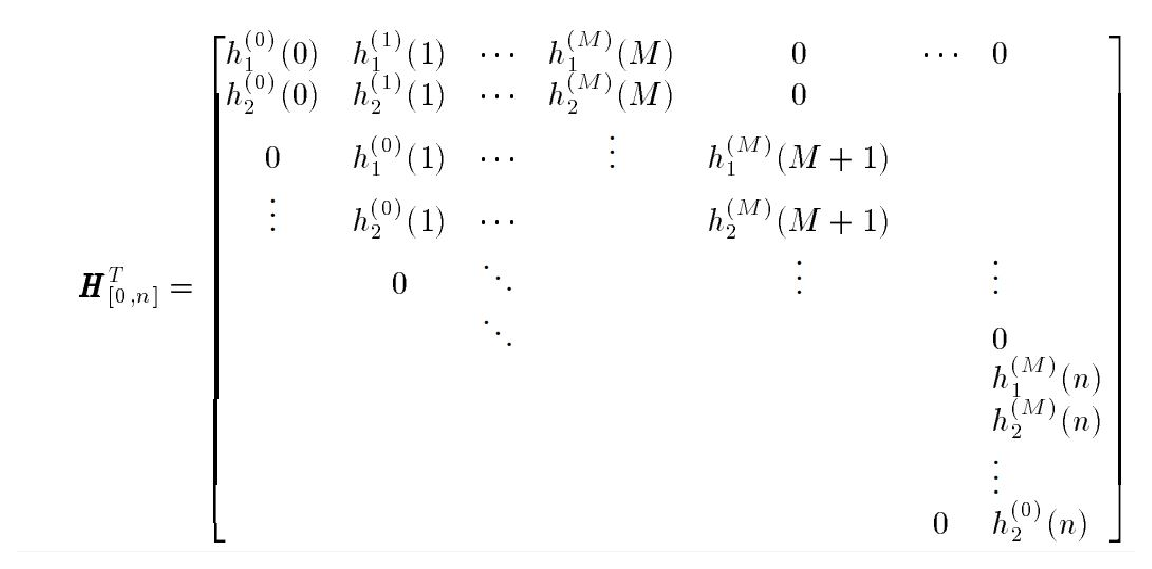
\includegraphics[width=0.55\textwidth]
		{\folder/eqn.eps}
		\label{fig1}
		\end{figure*}
	
	Since $h_1^{(0)}(n) = h_2^{(0)}(n) =1$. We find a sytematic encoder using the equation below
	
	\begin{equation}
\begin{aligned} v_{n, 1} &=u_{n} \\ v_{n, 2} &=\sum_{i=0}^{M} h_{1}^{(i)}(n) u_{n-i}+\sum_{i=1}^{M} h_{2}^{(i)}(n) v_{n-i, 2} \end{aligned}
\end{equation}

Generally, the encoder can be implemented using $c$ length $M+1$ shift registers in parallel and time varying connections from the register stages to the modulo 2 adders.


\section{Iterative Decoding of Low-Density Convolutional Codes}

It is assumed that a rate $1/2 ~ (M, 3(2), 5)$ ) low-density
time-varying periodical convolutional code is used for transmission
over the AWGN channel. The code symbols are modulated and mappedd to the signal points $w_n$ as 

\begin{equation}
\begin{array}{rlrl}{w_{2 n}} & {=1-2 v_{n, 1},} & {} & {n=0,1, \cdots} \\ {w_{2 n+1}} & {=1-2 v_{n, 2},} & {} & {n=0,1, \cdots}\end{array}
\end{equation}

The procedure is similar to that of the previous section. The major difference is the pipeline implementation of the decoder, which is made up of $I$ seperate processors and $J+1$ first-in-first-out FIFO shift registers. (FIFO). The first
register contains the log-likelihood metrics $\ell^{(1)}(n)$ received from the
channel, while the other $J$ registers contain intermediate statistics
computed by the different processors. Initially, the encoder contains
dummy zeroes. Therefore, the FIFO’s are initially filled with $1$,
which is the log-likelihood ratio for the absolute reliable received
statistics, which correspond to the code symbol zero. 

Each time a new channel statistic is received, it is shifted in all the
FIFO’s. Each statistic $\ell^{(1)}(n)$, flows through the FIFO, as in a pipeline,
and is processed sequentially by the $I$ processors. The $I$ processors are $2(M+1)$ registers apart from each other so they are processing different and consecutive segements of the FIFO stages.

 The decoding procedure is outlined below.
 \end{document}
